\subsubsection{GUI}
\label{subsec:gui}
La GUI intenta ser una manera más intuitiva de ejecutar el programa, sin necesidad de tener que ingresar todos los argumentos a mano. Se ejecuta (estando en la carpeta \textbf{src}) mediante el siguiente comando:

\begin{center}\textit{python3 gui/main.py}\end{center}\vspace{\baselineskip}

\begin{figure}[H]
    \centering
    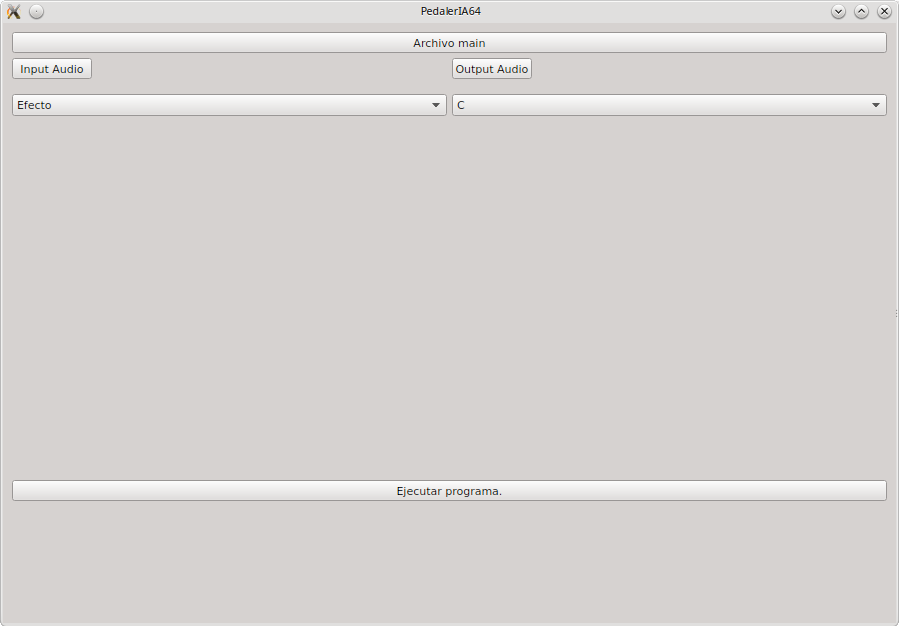
\includegraphics[scale=0.68]{imagenes/gui.png}
    \caption{GUI}
    \label{fig:gui}
\end{figure}

La GUI limpia se ve en la figura \ref{fig:gui}. Es necesario seleccionar dónde se encuentra el archivo \textbf{main}, el archivo de entrada sobre el cual se quiere aplicar el efecto, cuál es el nombre deseado del archivo de salida (se lo colocará en la misma carpeta donde se encuentra \textbf{main}) y, finalmente, el efecto a aplicar junto con sus argumentos.\vspace{\baselineskip}

La GUI con todos los argumentos completados, y luego de seleccionar el botón ``ejecutar programa'' se ve como en la figura \ref{fig:gui-complete}.\vspace{\baselineskip}

\begin{figure}[H]
    \centering
    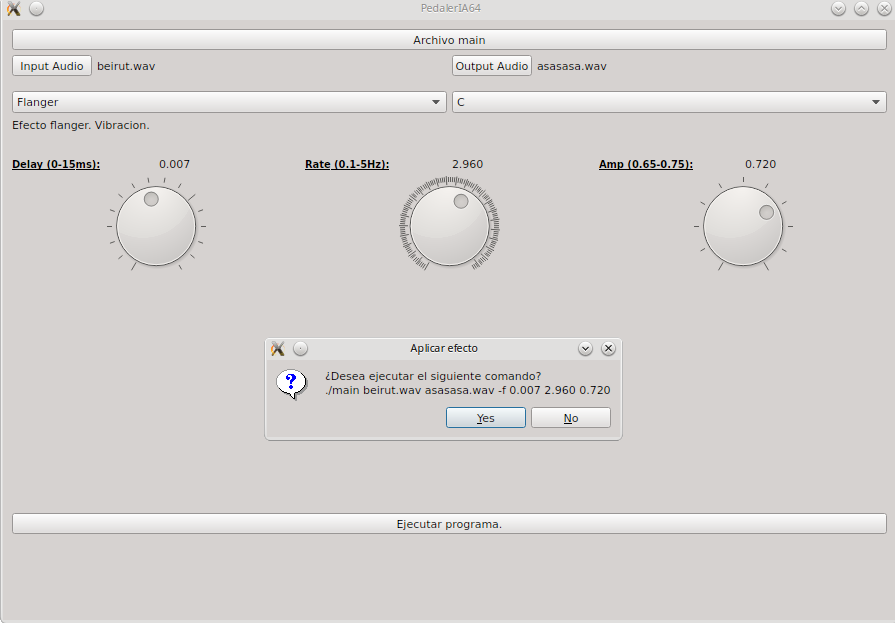
\includegraphics[scale=0.68]{imagenes/gui-complete.png}
    \caption{GUI con todas las opciones seleccionadas}
    \label{fig:gui-complete}
\end{figure}

\begin{center}
\fbox{\begin{minipage}{42em}
\underline{Nota}: En el popup para confirmar si el comando es el correcto, el mismo no representa exactamente lo que se ejecuta, pues faltan los paths hacia cada archivo. Para que no quede un texto largo e incomprensible en el popup, se decidió poner únicamente los nombres de los MAIN, INFILE y OUTFILE, aún cuando los primeros dos podrían no compartir carpeta (OUTFILE siempre está en la misma carpeta que MAIN).
\end{minipage}}
\end{center}\vspace{\baselineskip}

Al poner ``Yes'', la interfaz ejecutará el comando y, en caso de que todo haya salido correctamente, ofrecerá dos botones para poder reproducir el audio de entrada, el de salida, y comparar, como se puede ver en la figura \ref{fig:gui-play-buttons}.

\begin{figure}[H]
    \centering
    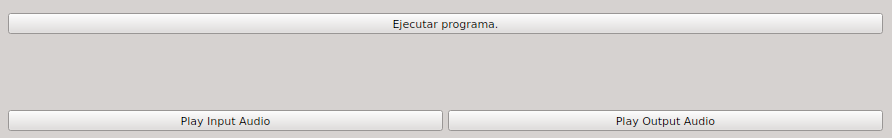
\includegraphics[scale=0.68]{imagenes/gui-play-buttons.png}
    \caption{Botones de reproducción}
    \label{fig:gui-play-buttons}
\end{figure}

En caso de que falle, se dará noticia de eso, pero no se manejará ni mostrará el error (se recomienda ejecutar el mismo comando que hubiera ejecutado la GUI en la CLI para ver qué pasó; de todos modos, es posible ver el error en la terminal desde donde se haya corrido Python).

En caso de que falte completar alguna opción, al hacer click en ``Ejecutar programa'' aparecerá un popup informando de cuál es la opción que falta llenar. 
